\documentclass[a4paper,11pt]{article}

\usepackage[english]{babel}
\usepackage[utf8]{inputenc}
\usepackage[vmargin=3.5cm,hmargin=2cm]{geometry}
\usepackage{graphicx}
\usepackage{caption}
\usepackage{subcaption}
\usepackage{amsmath}
\usepackage{mathtools}
\usepackage{fancyhdr}
\usepackage{listings}
\usepackage{makeidx}

\setlength{\footskip}{0cm}
\setlength\parindent{0pt}
\addtolength{\footskip}{0.8cm}
\addtolength{\headsep}{-.5cm}

\title{\bfseries Lab 2 \\}
\date{}

\lfoot{}
\cfoot{}
\rfoot{\textbf{Communication Systems} \\ Teresa Algarra Ulierte }

\renewcommand{\headrulewidth}{0.5pt}
\renewcommand{\footrulewidth}{0.5pt}

\begin{document}
\renewcommand\contentsname{\vspace{-1cm}}
\maketitle
\lstset{language=Matlab}

\begin{centering}
    Teresa Algarra Ulierte \\
    Student ID: teresaalgarraulierte \\
    Perm number: 7626872 \\
\end{centering}

\vspace{3cm}

\begin{figure}[!ht]
	\centering
	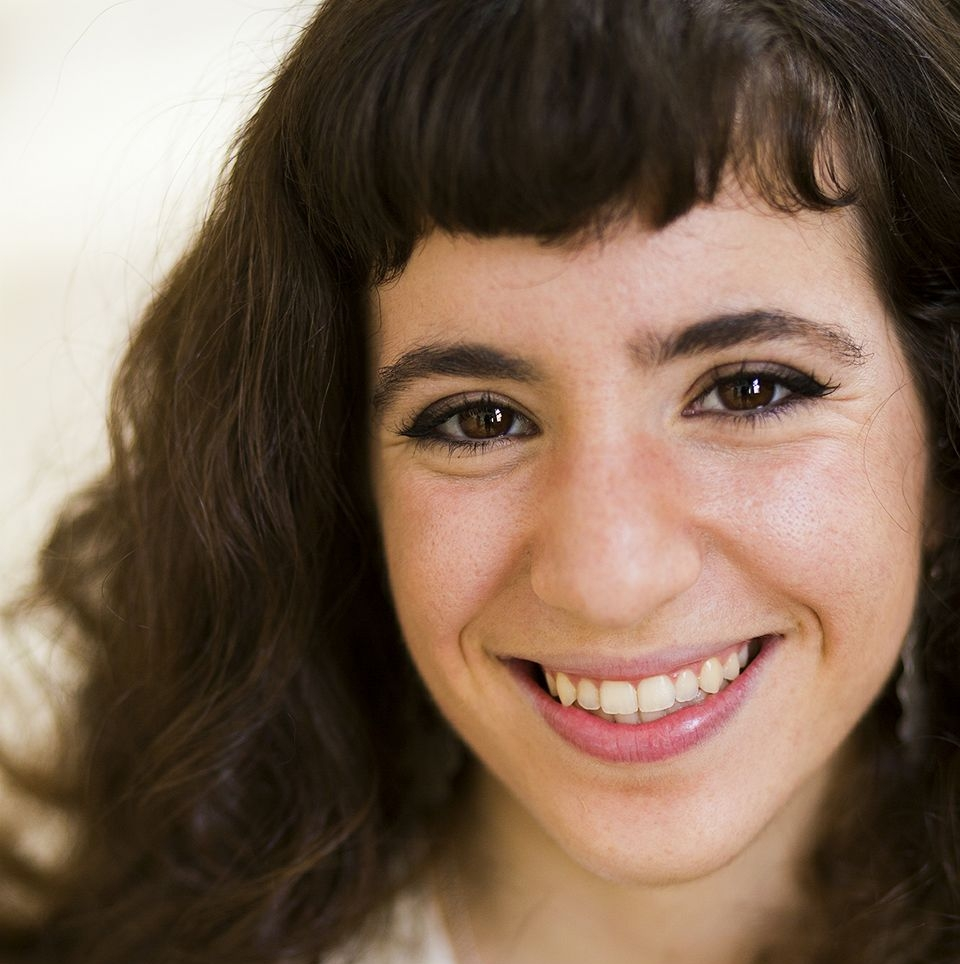
\includegraphics[scale = 0.25]{images/photo.jpg}
\end{figure}

\newpage

\section{Lab 2.2: Modeling Carrier Phase Uncertainty}

\subsection{Goal of the lab:}

The goal of this lab was to illustrate how wireless multipath channels can be
modeled in complex baseband.

\subsection{Laboratory assignment:}

For the first part I took a pair of independently modulated signals:

\bigskip

$u_c(t)=\sum_{n=1}^{N}b_c[n]p(t-n)$ and $u_s(t)=\sum_{n=1}^{N}b_c[n]p(t-n)$

\bigskip

where the symbols $b_c[n]$ and $b_s[n]$ are chosen with equal probability to be +1
or -1, and $p(t)=I_{[0,1]}(t)$.

\bigskip

For part 1.1, the plot for these two signals over 10 symbols was:

\begin{figure}[!ht]
	\centering
	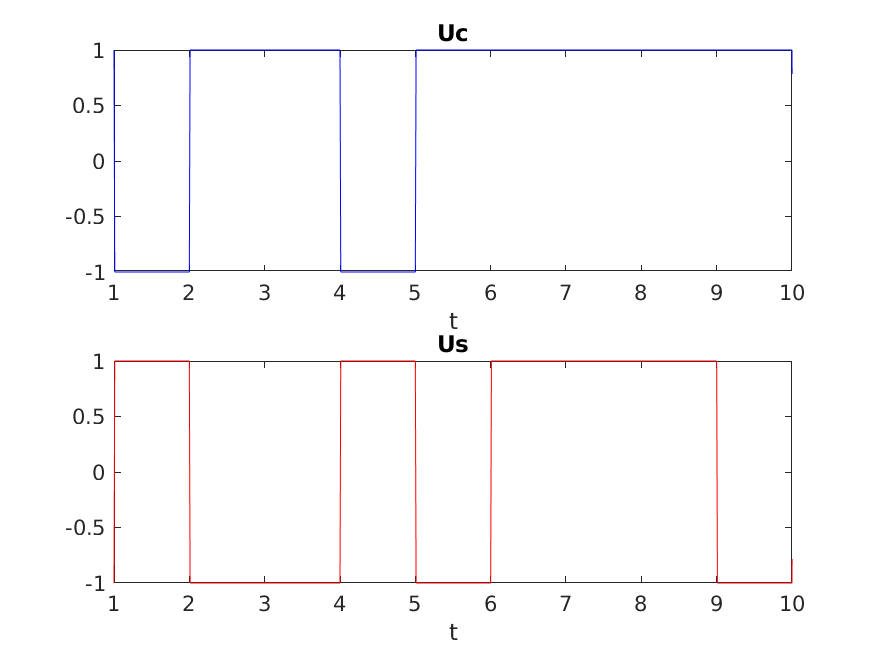
\includegraphics[scale = 0.6]{images/1_1.png}
\end{figure}

For part 1.2 I upconverted $u_c(t)$ by multiplying it by $cos(40\pi t)$. The
graph was a BPSK signal:

\begin{figure}[!ht]
	\centering
	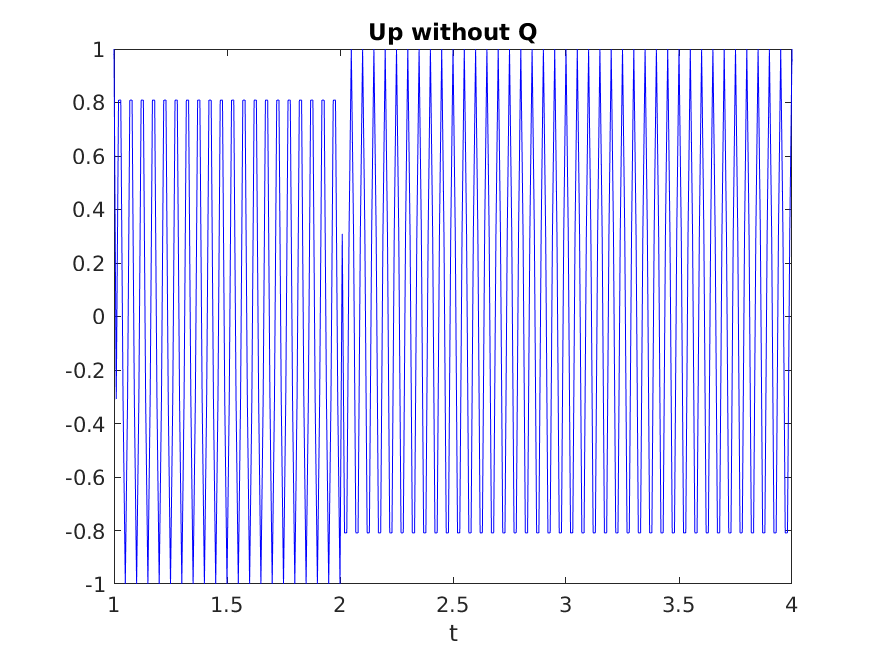
\includegraphics[scale = 0.6]{images/1_2.png}
\end{figure}

\newpage

That was the I component. To have the whole passband signal in 1.3, I had to add
the Q component, that is, $u_p(t) = u_c(t)cos(40\pi t) - u_s(t)sin(40\pi t)$. The
result is a QPSK signal:

\begin{figure}[!ht]
	\centering
	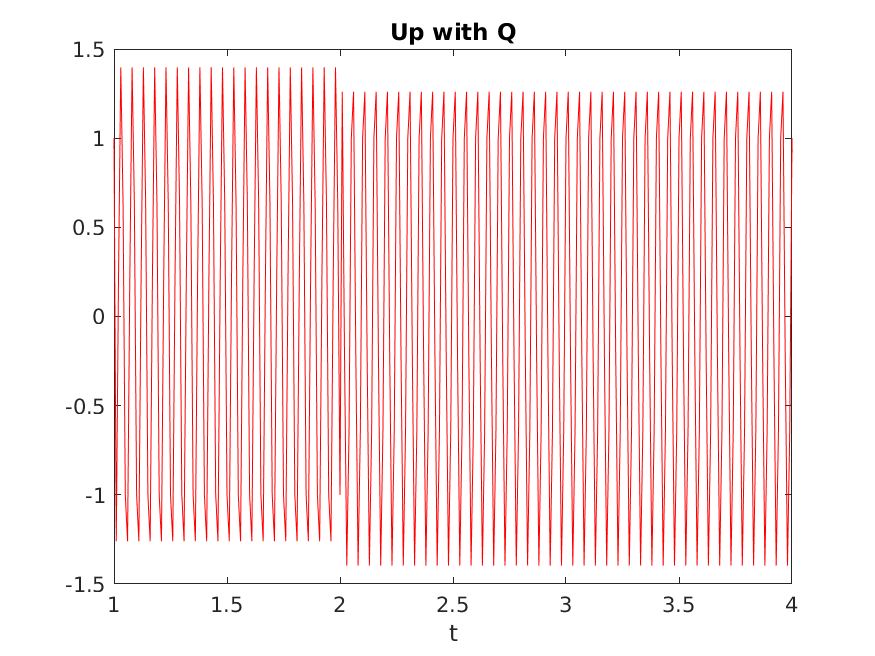
\includegraphics[scale = 0.8]{images/1_3.png}
\end{figure}

For part 1.4, I downconverted $u_p(t)$ by doing $2u_p(t)cos(40\pi t+\theta)$ and
$2u_p(t)sin(40\pi t+\theta)$ and then getting the resulting signals through a
low pass filter $h(t)=I_{[0,0.25]}(t)$. When $\theta = 0$, the result was:

\begin{figure}[!ht]
	\centering
	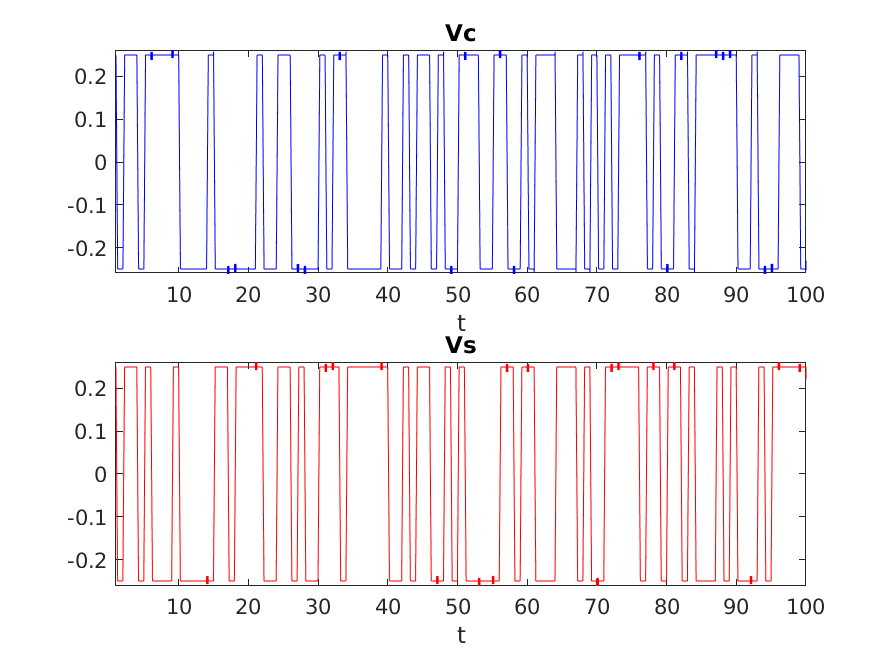
\includegraphics[scale = 0.8]{images/1_4.png}
\end{figure}

\newpage

On the other hand, when $\theta = \frac{pi}{4}$, the result was:

\begin{figure}[!ht]
  \centering
  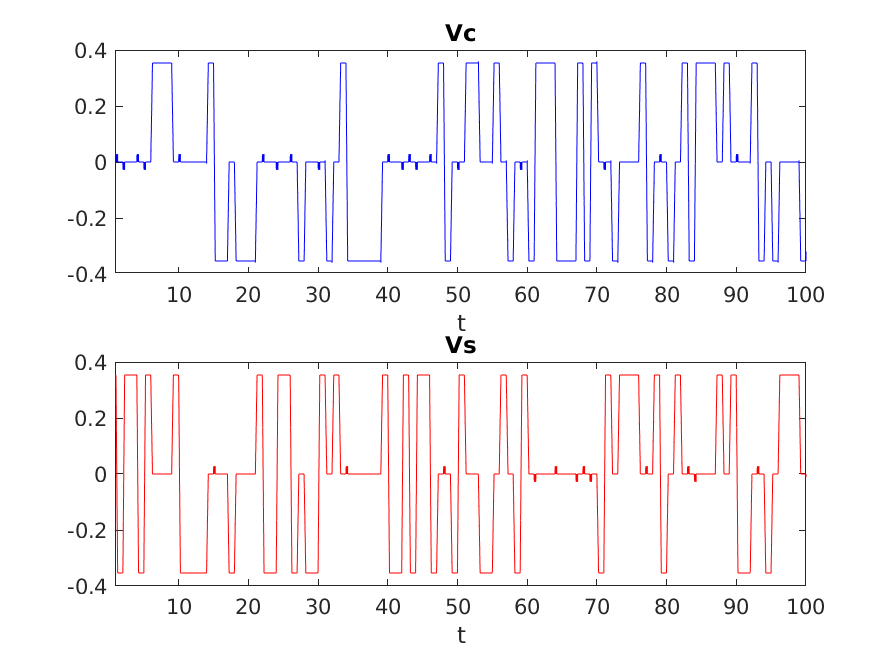
\includegraphics[scale = 0.8]{images/1_5.png}
\end{figure}

The result from part 2.5 was multiplied by $e^{-j\frac{pi}{4}}$. Then, to recover
$u_c(t)$ and $u_s(t)$ I had to multiply the outcome of part 2.5 by $e^{j\frac{pi}{4}}$.

\begin{figure}[!ht]
	\centering
	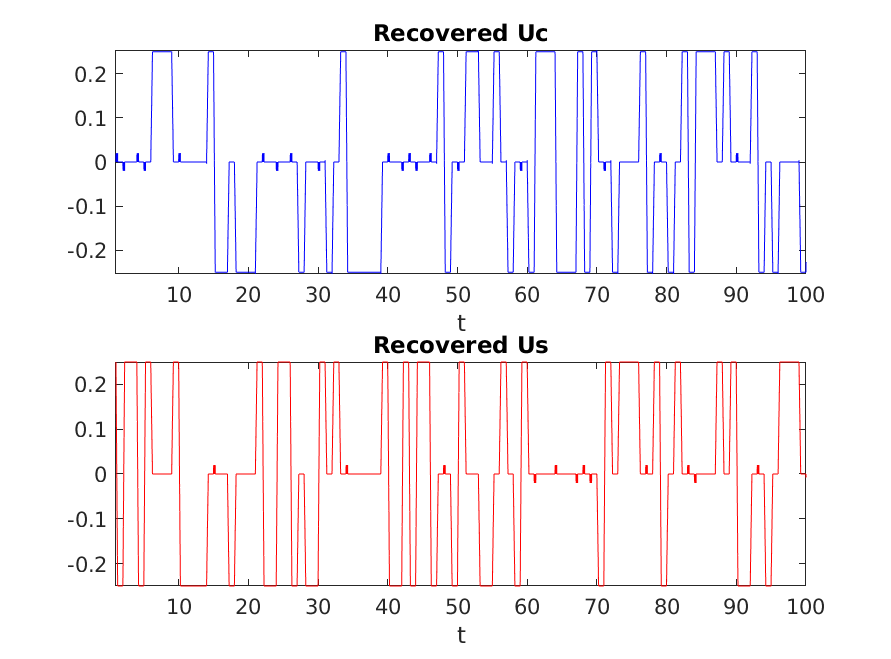
\includegraphics[scale = 0.8]{images/1_6.png}
\end{figure}

\newpage

Here there is a comparison between the recovered signals and the original ones.
One can see that now there are values in 0 that there weren't before because the
possible values were either -1 or +1. Now there are those in the middle because
when the phase was added, the QPSK constellation was shifted, adding some values.

\begin{figure}[!ht]
	\centering
	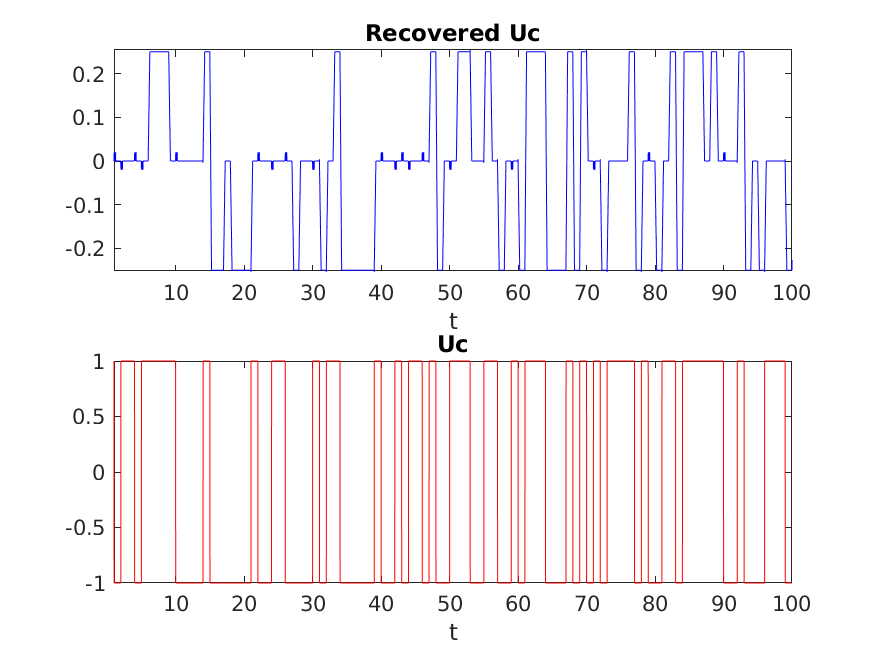
\includegraphics[scale = 0.8]{images/1_6a.png}
\end{figure}

\begin{figure}[!ht]
	\centering
	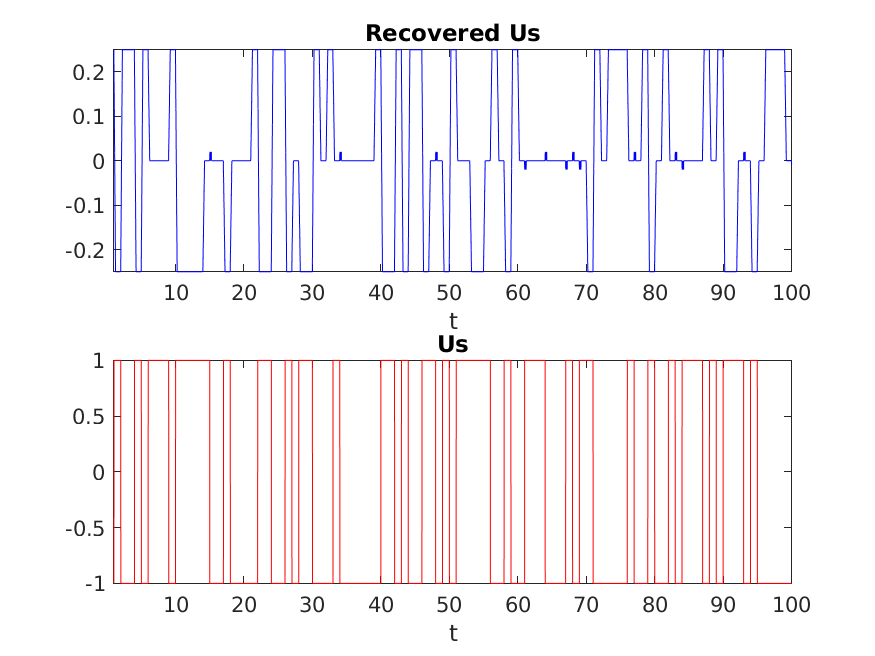
\includegraphics[scale = 0.8]{images/1_6b.png}
\end{figure}

\newpage

\section{Lab 2.3: Modeling a Lamppost based Broadband Network}

\subsection{Goal of the lab:}

The goal of this lab is to illustrate how wireless multipath channels can be
modeled in complex baseband, that is, the same as Lab 2.2.

\subsection{Laboratory assignment:}

The lab presents two lampposts of height 10 meters and separated 200 meters.
There is a direct path and an indirect path that works like in the figure:

\begin{figure}[!ht]
	\centering
	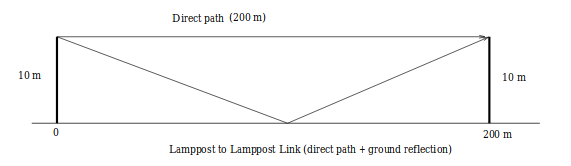
\includegraphics[scale = 0.8]{images/figure1.png}
\end{figure}

For 2.1, I had to find the delay spread and coherence bandwidth using
trigonometric formulas. The code used was:

\bigskip

\begin{lstlisting}

  f = 60e9;                                       %Unlicensed spectrum at 5GHz
  c = 3e8;                                        %Speed of light
  n1 = 1;                                         %Refractive index of air
  n2 = 8;                                         %Refractive index of ground
  D = 200;                                        %Distance between lampposts
  ht = 10;                                        %Height of the first lamppost
  hr = 10;                                        %Height of the second lamppost
  k = 2*pi*f/c;                                   %Wave Number
  d1 = sqrt(D.^2 + (ht-hr).^2);                   %Trigonometric formula
  d2 = sqrt(D.^2 + (ht+hr).^2);                   %Trigonometric formula

  delay = d2/c - d1/c;                            %Delay spread
  bc = 1/delay;                                   %Coherence Bandwidth

\end{lstlisting}

\bigskip

The resulting delay spread was 3.3250e-09, that is, 3.325 nanoseconds. On the
other hand, the coherence bandwidth was 3.0075e+08, that is, 0.3 Gigahertz.

If the message signal has 20 MHz bandwidth, the channel's coherence bandwidth is
more than 10 times the signal's bandwidth. Therefore, It can be considered
narrowband with respect to the channel.

\newpage

For 2.2 there is a car 2 meters tall and at 100m of the lamppost. The system is
modeled like in the figure:

\begin{figure}[!ht]
	\centering
	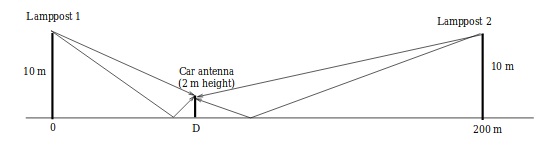
\includegraphics[scale = 0.8]{images/figure2.png}
\end{figure}

The code used is similar to the one above, so the resulting delay spread was
1.3265e-09, that is, 1.32655 nanoseconds. On the other hand, the coherence
bandwidth was 7.5389e+08, that is, 0.75 Gigahertz.

\bigskip

For 2.3 on I explored the sensitivity of the lamppost to lamppost sensitivity to
variations in height by varying the height of the receiver from 9.8m to 10.2m
in steps of 1mm. I plotted the normalized power gain in dB, that is,
$20log_{10}\displaystyle\frac{|h|}{|h_{nom}|}$ with the following result:

\begin{figure}[!ht]
	\centering
	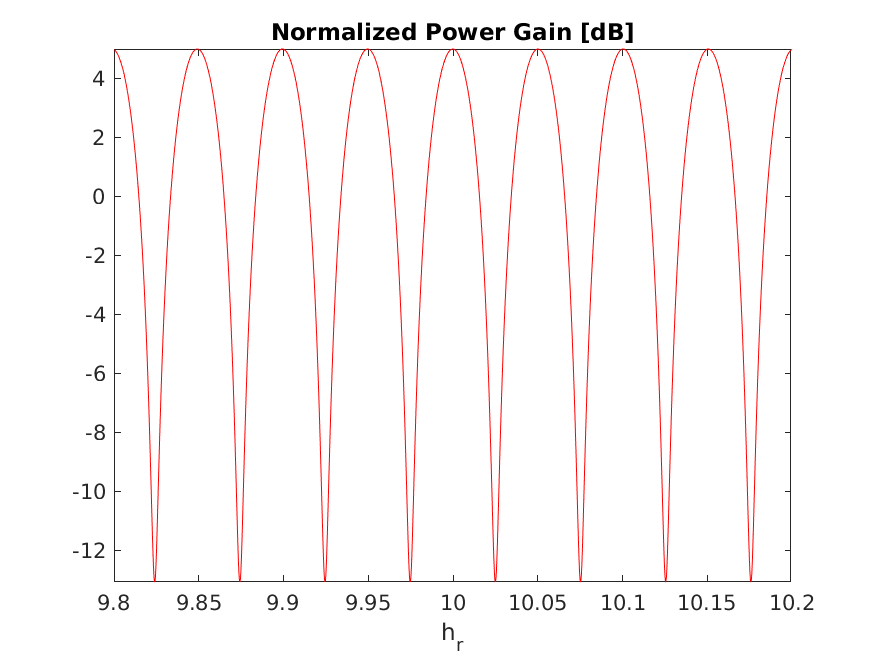
\includegraphics[scale = 1]{images/2_3.png}
\end{figure}

The NPG is maximum every 0.05m in multiples of 5, and minimum every 0.05m but
right in the middle of all the maximums.

\newpage

For 2.4 I calculated the probability of the normalized power gain being smaller
than -10dB. Since we have an uniform distribution, this could be done by
dividing the number of point in which this happens by the total number of points.

\bigskip

\begin{lstlisting}

  i = 0;                                          %Counter
  for x = 1:length(npg1)                          %Going through npg1
      if npg1(x) <= -10                           %Condition
          i = i+1;                                %Adding counter
      end                                         %End of conditional loop
  end                                             %End of for loop

  probability = 100*i/length(npg1);               %Probability in %

\end{lstlisting}

\bigskip

The resulting probability is 8.1480\%.

\bigskip

For 2.5 we have to repeat exercise 2.3, but now there are two antennas
vertically spaced by 1cm, that is, one at 10m and the other one at 10.1m.
Therefore we get two plots for the normalized power gain, one for the lower
antenna and one for the upper antenna. The result is:

\begin{figure}[!ht]
	\centering
	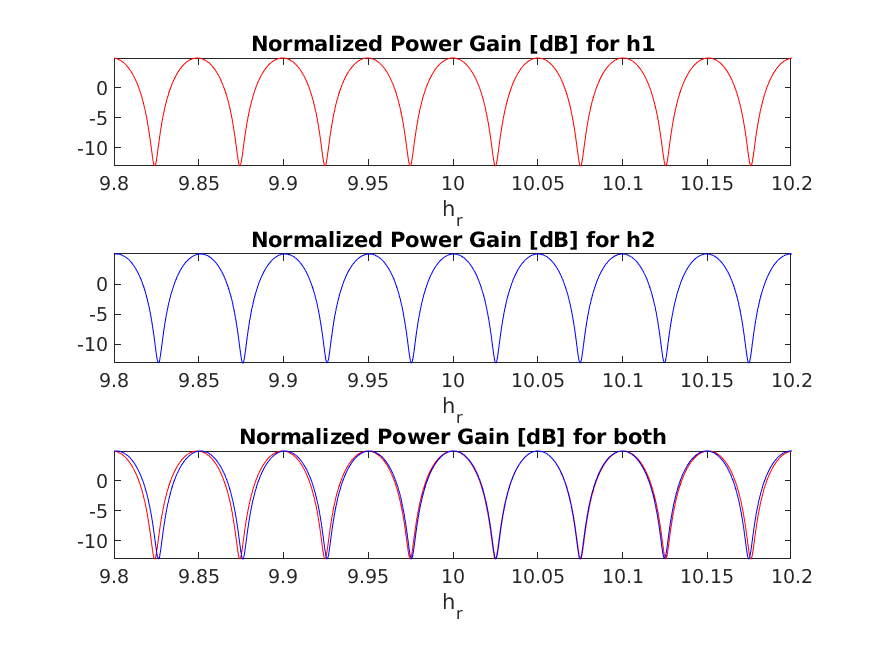
\includegraphics[scale = 1.05]{images/2_5.png}
\end{figure}

The peaks look like they are almost at the same time all the time looking at
teh two first figures, but as one can see in the third figure, they are not
quite at the same time. They are only exactly the same between 10.025 and 10.075
and they have a phase elsewhere.

\newpage

For 2.6 I plotted the normalized power gain for the antenna whose channel is
better with $20log_{10}\displaystyle\frac{max(|h_1|,|h_2|)}{|h_{nom}|}$. The
result was the plot for the upper antenna:

\begin{figure}[!ht]
	\centering
	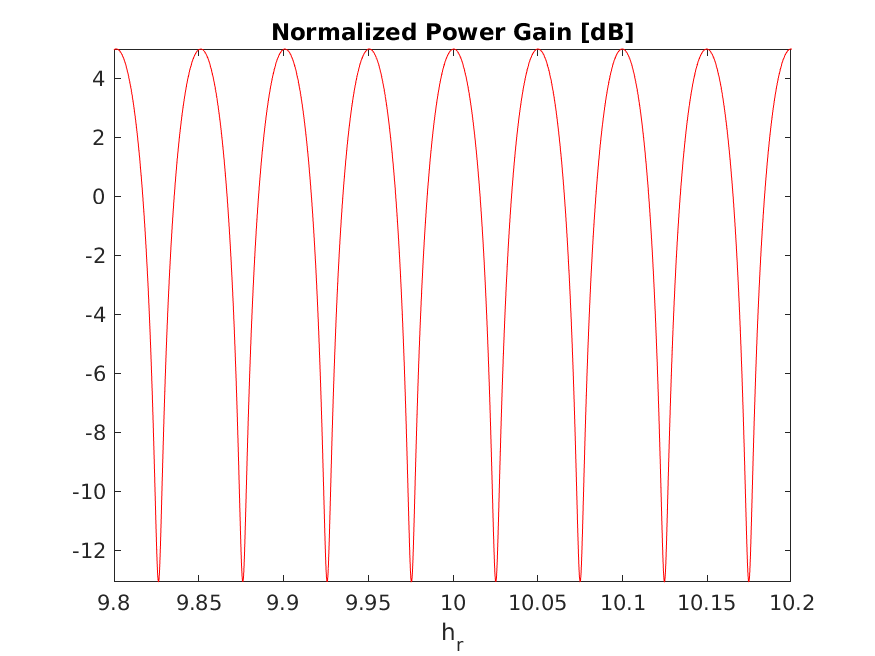
\includegraphics[scale = 0.7]{images/2_6.png}
\end{figure}

Now the minimum value is -13.06dB.

\bigskip

For 2.7 I had to calculate the probability of the graph in 2.6 being lower than
-10dB. I used the same code as in 2.4, with a final probability of 8.0980\% of the
values dropping under -10dB as opposed to a probability of 8.1480\% for the lower
antenna, that is, 0.05\% higher probability for the lower antenna.

\bigskip

For 2.10 I worked with frequency diversity. I worked with the original heights
of the lampposts to get the normalized channel as a function of the carrier frequency
using a vector from 59GHz to 64GHz with a step size of 10MHz. The normalized channel
plot was:

\begin{figure}[!ht]
	\centering
	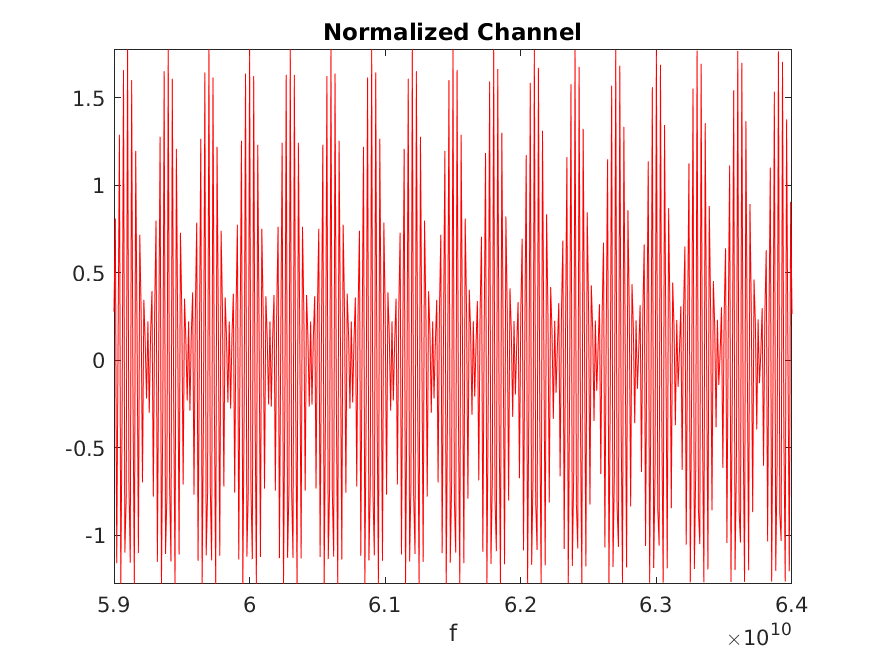
\includegraphics[scale = 0.7]{images/2_10.png}
\end{figure}

For 2.11 I had to calculate the probability of the normalized channel gain
being below -10dB if the carrier frequency is chosen randomly over $[59, 64]$ GHz.
I used the same code as in 2.4 and 2.7, with a final probability of 7.3852\%.
The normalized power gain of this normalized channel with random frequency is the
following:

\begin{figure}[!ht]
	\centering
	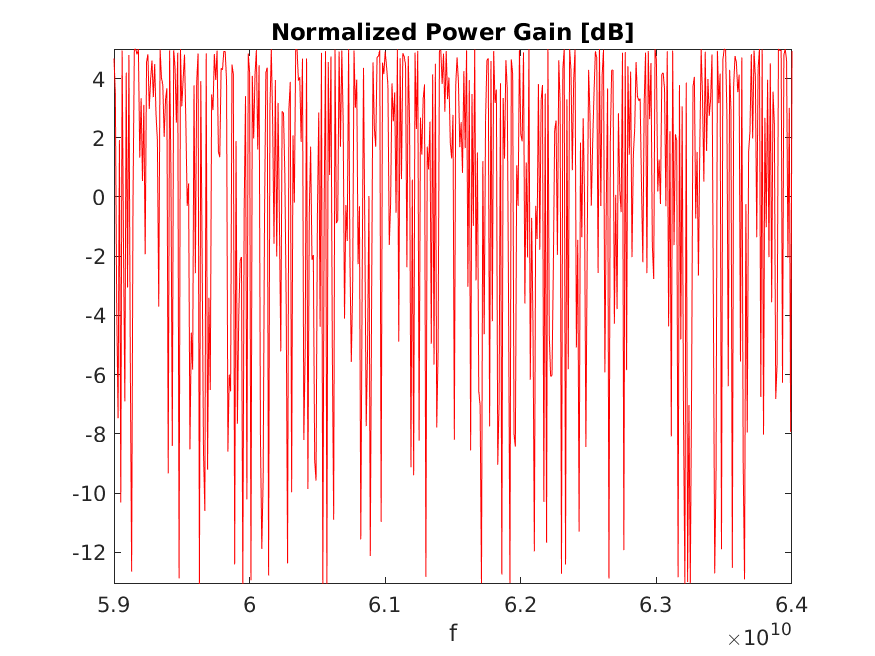
\includegraphics[scale = 0.8]{images/2_11.png}
\end{figure}

For 2.14 I worked with $|h_{nom}|$ and $|h|$ as functions of the distance, coming
back to the access channel from the lamppost to the car. I plotted how the
amplitude in dB decays with the distance from $1$ to $500m$ with the following result:

\begin{figure}[!ht]
	\centering
	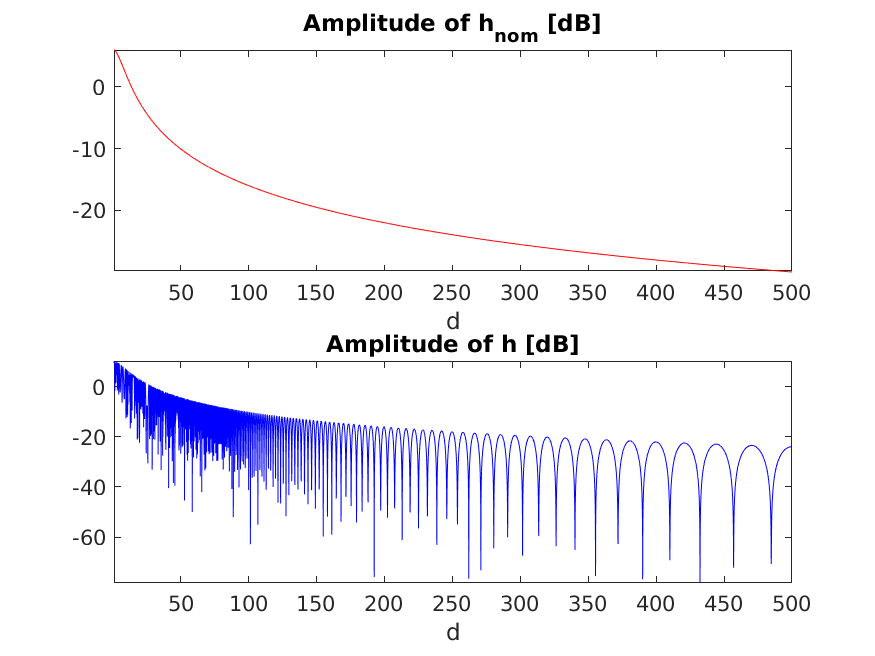
\includegraphics[scale = 0.8]{images/2_14a.png}
\end{figure}

As one can see, it decays faster in the beginning and the the curve smooths. When
zooming in to the first values, one can appreciate it:

\begin{figure}[!ht]
	\centering
	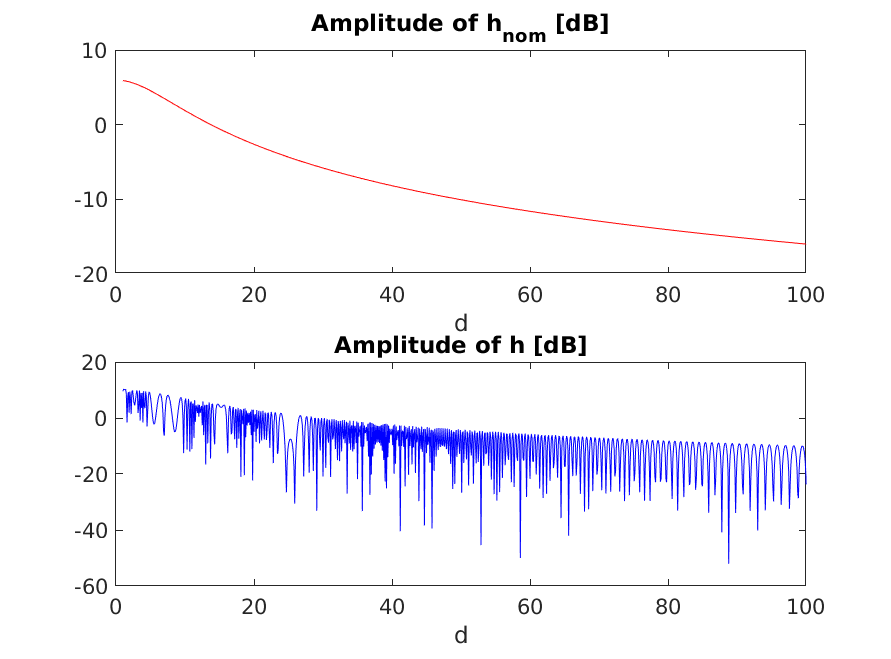
\includegraphics[scale = 0.85]{images/2_14b.png}
\end{figure}

Finally, 2.15 consists of repeating 2.14 but taking in count the effect of
surface roughness, that is, taking $A_r = \alpha_{s}\rho_s$ with
$\alpha_{s} = e^{-8(\pi \sigma cos(\theta_{i}/\lambda)^2}$. The plot obtained was:

\begin{figure}[!ht]
	\centering
	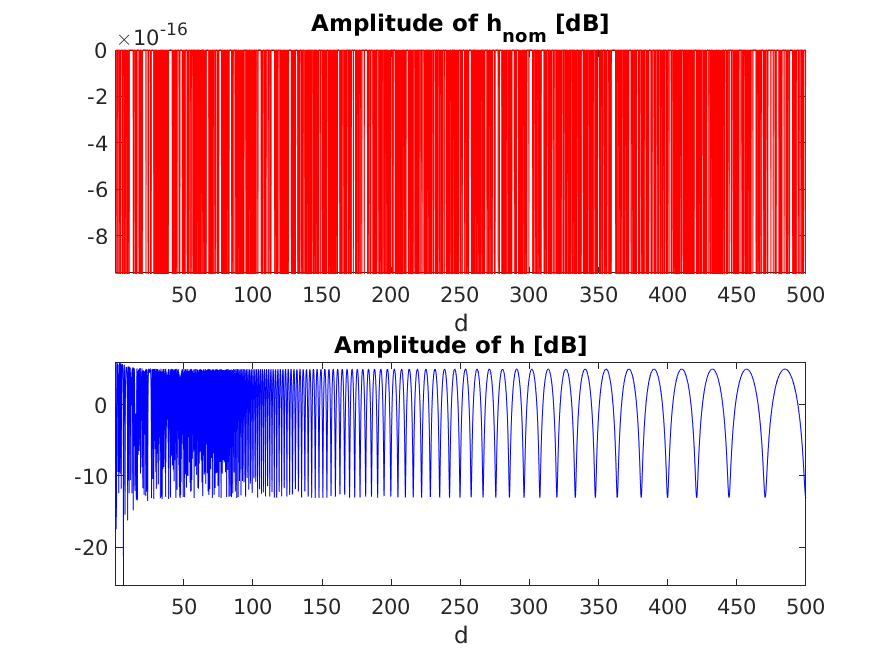
\includegraphics[scale = 0.85]{images/2_15a.png}
\end{figure}

\newpage

Here the amplitude stays constant for all the distance. When zooming in to the
first values, one can see that they don't change:

\begin{figure}[!ht]
	\centering
	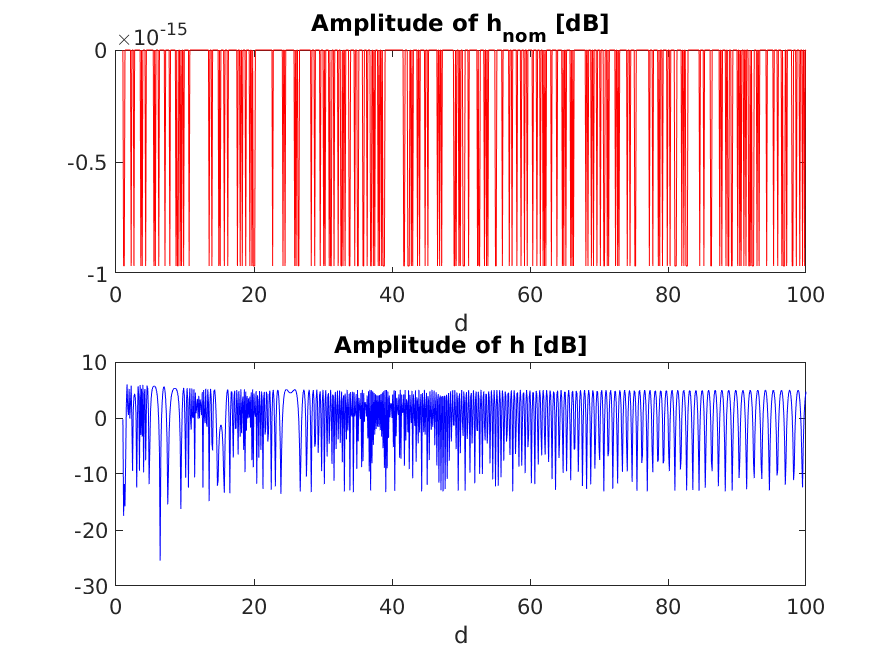
\includegraphics[scale = 0.8]{images/2_15b.png}
\end{figure}

\section{Conclusion:}

In this lab I learned how to use MatLab to work with complex baseband (Lab 2.2)
and with multipath channels (Lab 2.3). I felt like Lab 2.2 was a bit smoother to
do, partly because it did not involve any trigonometry and it was only working with
pure signals. Lab 2.3 was definitely harder, as well as longer. It was really
helpful to see how parameters like the amplitude or the sensitivity change with
others like the frequency, the distance between two antennas or the distance.
Unfortunately, I was not able to finish exercises 2.8, 2.9, 2.12 and 2.13, since I
did not understand what was being asked in the question and I could not reach
out for help in time to hand it in. Nevertheless, I will ask in the next lab
session to make sure I understand everything about multipath channels and how
they behave. Overall, I think now I understand better the second half of chapter
2 of the book and I am better prepared to work with problems in this area.

\vspace{4cm}

\end{document}
